\section{Optimising Abstract Graph Size}
\par \indent
As we have observed in lemmas \ref{aha-lemma:maxedgesincluster} and \ref{aha-lemma:maxtransitions} the initial abstraction algorithm attempts to represent every optimal path between clusters and inside clusters.
However, most maps have far simpler topographies than the worst-case; in our  experimental scenarios we often observed the same path returned for different pairs of $(c, s)$ parameters when discovering intra-edges.
This observation presents us with an opportunity to compact the graph and reduce the associated space complexity of our decomposition technique. 
We achieve this by noticing that if several optimal-length edges exist between two nodes, annotated with the same capability but with different clearance values, we can discard all edges except the one with the largest clearance. 
\par \indent
Consider the initial abstraction in Figure \ref{aha-fig:strongdominance}(a) and contrast it with our desired result in Figure \ref{aha-fig:strongdominance}(b). $\lbrace E3, E5 \rbrace$ represent the same path between nodes $b$ and $c$ but are annotated with different clearance values. 
The same problem is evident for $\lbrace E4, E6 \rbrace$ which both cover nodes $a$ and $c$. In such cases we say that $E3$ and $E4$ are \emph{strongly dominant}, which we denote $E3 \prec E5$ and $E4 \prec E6$. We give the following theorem to formalise this concept:

\begin{theorem}
\label{aha-definition:strongdominance}
Let $e_{a}, e_{b} \in E_{abs}$ be two edges that connect the same pair of abstract nodes such that:
$$ 1 \geq e_{a}(c) \geq e_{b}(c) \wedge weight(e_{a}) \leq weight(e_{b})$$
Then $e_{a} \prec e_{b}$ and we may remove $e_{b}$ from $E_{abs}$ without loss of generality or optimality.
\end{theorem}
\begin{proof}
Any agent able to traverse an edge with small clearance is also able to traverse another edge with larger clearance. Since both $e_{a}$ and $e_{b}$ have the same weight we lose neither optimality nor generality by removing $e_{b}$.
\end{proof}
We term the resultant graph in which all strongly dominant edges have been removed a \emph{high-quality} abstraction.  

\begin{figure}[htbp]
        \caption{\emph{Strong edge dominance} }
        \begin{center}
                        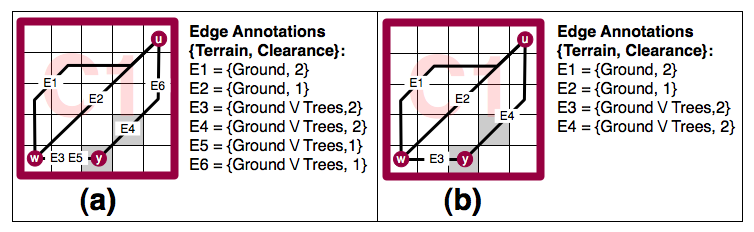
\includegraphics[scale=0.3]{diagrams/intraedges_initial.png}
        \end{center}
        \label{aha-fig:strongdominance}
\end{figure}

The abstract graph can be further reduced by noticing that some multi-terrain transitions between clusters can be removed without affecting the completeness of the representation. 
Figure \ref{aha-fig:abstractgraph}(a) and (b) highlight the problem and \ref{aha-fig:abstractgraph}(c) and (d) the desired outcome.
\begin{figure}[htbp]
        \caption{\emph{High and low quality abstraction results} }
        \begin{center}
                        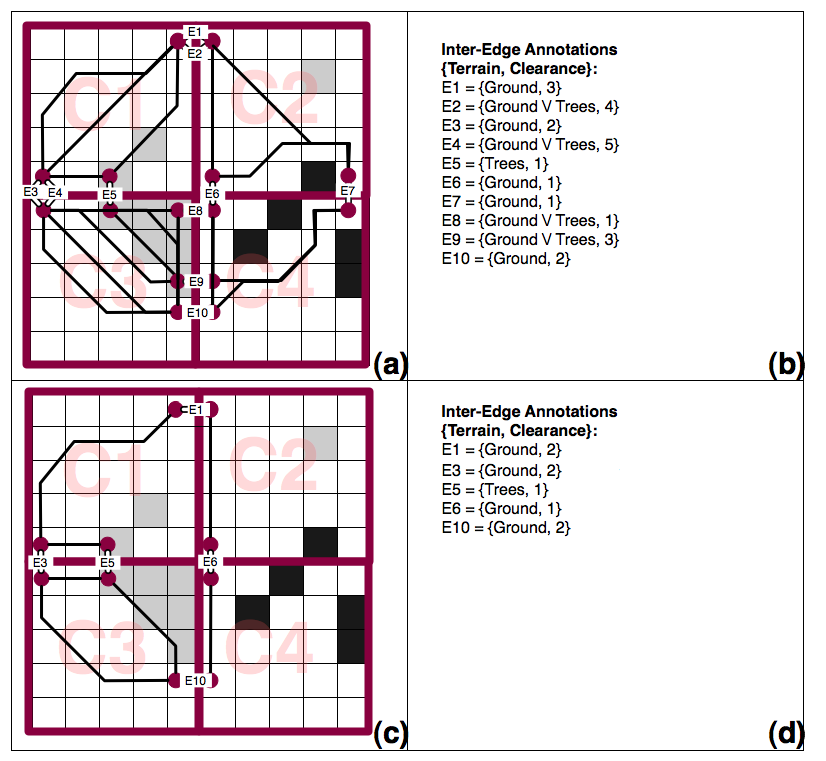
\includegraphics[scale=0.25]{diagrams/abstraction_result.png}
        \end{center}
        \label{aha-fig:abstractgraph}
\end{figure}
\par \indent
In this example we can see that although edges $E1$ and $E2$ have different clearance values any agent of size $s \in S : S = \lbrace 1, 2 \rbrace$ capable of traversing $E2$ can also traverse $E1$ without loss of generality. 
In such cases we say $E1$ is \emph{weakly dominant} and denote it as $E1 \sim E2$. 
We may further notice that $E3 \sim E4$, $E6 \sim E7$, $E10 \sim E8$ and $E10 \sim E9$ which suggests we can safely remove the dominated edges without losing any connectivity information from the graph. 

We formalise the concept using the following theorem:
\begin{theorem}
\label{aha-theorem:weakdominance}
Let $\lbrace n1_{a}, n2_{a} \rbrace, \lbrace n1_{b}, n2_{b} \rbrace \in V_{abs}$ denote two sets of abstract nodes in two adjacent clusters $\lbrace L_{1}, L_{2} \rbrace$. Suppose each node set is respectively connected by one of two inter edges $e_{a}, e_{b} \in E_{abs}$ with clearance values $e_{a}(c_{a}), e_{b}(c_{b})  : c_{a} \in c_{b} \in C$.
 In this scenario, $e_{a} \sim e_{b}$ iff the following conditions are met:
\begin{enumerate}
\item{The capability dominance condition: $e_{a}(c_{b}) \geq e_{b}(c_{b})$}
\item{The circuit condition: $\exists intra_{1}, intra_{2} \in E_{abs} : \lbrace n1_{a}, n1_{b} \rbrace \in intra_{1} \wedge \lbrace n2_{a}, n2_{b} \rbrace \in intra_{2} \wedge intra_{1}(c_{b}) \geq e_{b}(c_{b}) \wedge intra_{2}(c_{b}) \geq e_{b}(c_{b})$.}
\end{enumerate}
Then, any location which an agent can reached by traversing $e_{b}$ can also be reached by $e_{a}$.
\end{theorem}

\begin{proof}
If a circuit exists between the endpoints $\lbrace n1_{a}, n2_{a}, n1_{b}, n2_{b} \rbrace$ which contains only edges with clearances at least as large as $e_{b}(c_{b})$ for the capability $c_{b}$ then any nodes which are reachable from $n1_{b}$ or $n2_{b}$ are also reachable from $n1_{a}$ or $n2_{a}$.
From this it follows that any destination an agent can reach via $e_{b}$ can also be reached via $e_{a}$ 
\end{proof}
\begin{corollary}
If $e_{a} \sim e_{b}$, then $n1_{b}$ and $n2_{b}$ and are also dominated and can be removed, unless required by another (non-dominated) inter-edge. 
\end{corollary}
\begin{proof}
If $n1_{b}$ and $n2_{b}$ are required by a non-dominated inter-edge we cannot remove them without violating the capability dominance condition which is required to retain representational completeness. 
If this is not the case however, we know by the circuit condition that any node reachable by an intra-edge via $n1_{b}$ or $n2_{b}$ is reachable via the endpoints of $e_{a}$. 
Thus, both nodes and any associated intra-edges dependent on them, can be safely removed.
\end{proof}
Of course, opting for a low-quality abstraction in this way does affect the quality of computed solutions. 
In the worst case, a one-step transition of cost 1.0 in a high quality graph may be as long as $n \times 6$, where $n$ is the length of a cluster in a low-quality approximation.
This is a pathological case however; as we will show the differences in real-world scenarios are much smaller and still near-optimal. 
The choice of which quality abstraction technique to employ will depend on the requirements of the specific application to which the algorithm is applied.
It is a classic tradeoff between run-time performance vs space.
